\subsection{GNNs for Atomic Simulations}
\label{subsec:atomic-simulations}

\subsubsection{General}

Suppose one has information about the chemical and spatial structure of a molecule 
and would like to predict properties of this very molecule, e.g. its energy (at the 
current point in time or after some evolution) or the forces acting on the 
individual atoms. Some of these properties might be directly
computable using quantum mechanical methods---like Density Functional Theory (DFT) 
\cite{doi:10.1021/ed5004788}, inter alia
to compute bond energies in molecules. However, these methods often come
with significant drawbacks as they might be extremely expensive from a computational 
standpoint, imposing the necessity to either optimize these conventional methods 
as far as possible or use completely different approaches.

One alternative approach that is subject to current research is to compute or 
predict such molecule properties using supervised
machine learning in order to learn a function that maps molecule structures to their
respective properties based on data of known molecules. For this task, Graph
Neural Networks (GNNs) are very well suited not only because a molecule can naturally
be expressed as a graph (e.g. using its structural formula with atom numbers and
interatomic distances as node and edge attributes), but also because in this case, the 
assumption of invariance w.r.t. permutations of the atoms or the assumption that 
the update rules do not differ between nodes or edges and that one is hence
learning somewhat universal functions, seem very reasonable.

From now on, we define a molecule consisting of $n$ atoms by its atomic numbers 
$\zz$ and its positions $\XX$, where
\begin{equation}
    \XX \: \coloneqq \: \set{\xx_1, \dots, \xx_n}, \; \xx_i \in \R^3
    \qquad \text{and} \qquad 
    \zz \: \coloneqq \: \set{z_1, \dots, z_n}, \; z_i \in \N \text{.}
    \label{eq:molecule_setup}
\end{equation}
Nonetheless, in many cases there is still some arbitrariness in the choice of the 
exact positions $\XX$: Energies of molecule structures might be invariant w.r.t. 
translations and rotations, or forces might be invariant w.r.t. 
translations and equivariant w.r.t. rotations. Rather than letting the model figure out
these fundamental invariants of its predicting function learn on its own (e.g. by 
data augmentation), they are often directly incorporated into the model to reduce 
complexity. One approach to achieve this is to compute pairwise distances $d_{ij}$ 
between the atoms and use them instead of the individual atomic locations $\XX$, 
so---in the GN language (see \ref{subsubsec:gns})---define an input graph with the atomic numbers $\zz$ as 
node attributes and the interatomic distances as edge attributes (say, if a bond exists
between two atoms or if the distance is below some threshold). However, this might
not always be sufficient to completely characterize the spatial structure of a molecule:
Since the interatomic distances are only kept for a part of the pairs of 
nodes, there exist pairs of different molecules which cannot be
distinguished with this approach \cite[Appendix A]{DBLP:journals/corr/abs-2003-03123}.
Gasteiger et al. proposed multiple GNN architectures which overcome this
problem: DimeNet \cite{DBLP:journals/corr/abs-2003-03123} and 
DimeNet++ \cite{https://doi.org/10.48550/arxiv.2011.14115} achieve this
by incorporating directional information as bond angles into the models
(i.e. triplets of nodes), while in a more recent architecture, GemNet 
\cite{https://doi.org/10.48550/arxiv.2106.08903}, even 4-way interactions are
modeled.

\subsubsection{DimeNet and DimeNet++}
\label{subsubsec:dimenet}

DimeNet (\enquote{Directional Message Passing Neural Network}) 
\cite{DBLP:journals/corr/abs-2003-03123}, which was proposed by Gasteiger et al. 
in 2020, is an energy-centric GNN architecture for predicting energies and forces 
of molecule structures. DimeNet does not only consider pairwise distances between atoms, 
but also takes advantage of directional information. In the EGN 
language (see \ref{subsubsec:egns} and \cite{https://doi.org/10.48550/arxiv.2203.09697}),
3-way interactions between nodes are modeled.

Just as in \eqref{eq:molecule_setup}, the network receives the positions $\XX$
and atomic numbers $\zz$ of a molecule as inputs. 
At first, define the pairwise distances and relative direction vectors
\[
    d_{ij} \: \coloneqq \: \norm{\xx_j - \xx_i}_2, 
    \qquad \vec{\xx}_{ij} \: \coloneqq \xx_j - \xx_i \text{.}
\]
In the beginning, a molecular graph is given or it is defined by connecting the atoms with distance 
below some threshold $c$. Denote by $\mathcal{N}_i \subseteq \set{1, \dots, n}$ the 
neighborhood of the atom $i$.
Directional information is now leveraged by also 
taking the angles
\[
    \alpha_{kji} \: \coloneqq \: \measuredangle\left( \vec{\xx}_{jk}, \vec{\xx}_{ji} \right)
\]
between neighboring edges $(\_,k,j)$ and $(\_,j,i)$ into account. 
The distances and angles are then transformed to a representation which is related
to DFT calculations \cite[Section 5]{DBLP:journals/corr/abs-2003-03123}
by using radial and spherical Bessel functions:
\[
    \ee_{\text{RBF}}^{(ji)} \: \coloneqq \: \ee_{\text{RBF}}(d_{ji}), 
    \qquad \aaa_{\text{SBF}}^{(kji)} \: \coloneqq \: \aaa_{\text{SBF}}(d_{kj}, \alpha_{kji})
    \text{.}
\]
In an embedding phase, edge embeddings $\mm_{ji}^{(1)}$ and outputs
$t_{i}^{(1)}$ or a global attribute $t^{(1)} = \sum_{i=1}^n t_i^{(1)}$ are initialized based
on the atomic numbers $\zz$ and $\ee_{\text{RBF}}^{(ji)}$. Both node embedings 
$\hh_i \coloneqq \sum_{j \in \mathcal{N}_i} \mm_{ji}$ and triplet embeddings are handled
implicitly (i.e. the \textbf{Triplet Update} and \textbf{Node Update} outputs from 
\ref{subsubsec:gns}, \ref{subsubsec:egns} do not depend on their respective predecessors).
From now on, we denote implicit or irrelevant embeddings by \enquote{$\_$}.

In the EGN language, the initial graph is defined as follows:
\[
    G \: = \: (t^{(1)}, V^{(1)}, E^{(1)}, T^{(1)})
\]
with nodes, edges and triplets
\begin{align*}
    V^{(1)} \: &\coloneqq \: \setcomp{\hh_i^{(1)}}{i \in \set{1, \dots, n}}, \\
    E^{(1)} \: &\coloneqq \: \setcomp{(\mm_{ji}^{(1)}, i, j)}
    {i, j \in \set{1, \dots, n}, d_{ji} \leq c}, \\
    T^{(1)} \: &\coloneqq \: \setcomp{(\_,(\mm_{kj}^{(1)}, j, k), (\mm_{ji}^{(1)}, i, j))}
    {i, j, k \in \set{1, \dots, n}, \; d_{ji}, d_{kj} \leq c} \text{;}
\end{align*}
i.e. the triplets are all possible paths of length two on the edges of $G$.

After this initial graph embedding has been computed, a series of EGN blocks,
here called \textit{interaction blocks}, are applied to the graph.

Within such an interaction block, the edge embeddings 
are updated as follows (i.e. corresponds to \textbf{Edge Update}):
\[
    \mm_{ji}^{(l+1)} \: = \: 
    f_{\text{update}}\Bigg(\mm_{ji}^{(l)}, 
    \underbrace{\sum_{k \in \mathcal{N}_{j} \backslash\{i\}}}_{\textbf{Triplet Aggr.}} 
    \underbrace{ \vphantom{\sum_{\mathcal{N}_j}} 
    f_{\text {int }}\left(\mm_{k j}^{(l)}, \ee_{\text{RBF}}^{(ji)}, 
    \aaa_{\text{SBF}}^{(kj, ji)}\right)}
    _{\textbf{Triplet Update}}\Bigg) \text{,}
\]
where $f_{\text{int}}$ and $f_{\text{update}}$ are implemented by neural networks.
These edge embeddings are then directly aggregated to the new node embeddings
\[
    \hh_i^{(l+1)} \: = \: \sum_{j \in \mathcal{N}_i} \mm_{ji}^{(l+1)}
\]
and the outputs $t^{(l+1)}_i$ as well as the global attribute $t^{(l+1)}$ are
updated (based on another \textbf{Edge Aggregation} step).
Finally, the global output $t$ that represents the molecule's energy is 
aggregated over all interaction block outputs.
The whole DimeNet architecture as depicted in its original paper 
\cite{DBLP:journals/corr/abs-2003-03123} can be seen in Figure~\ref{fig:dimenet}.

\begin{figure}[H]
    \centering
    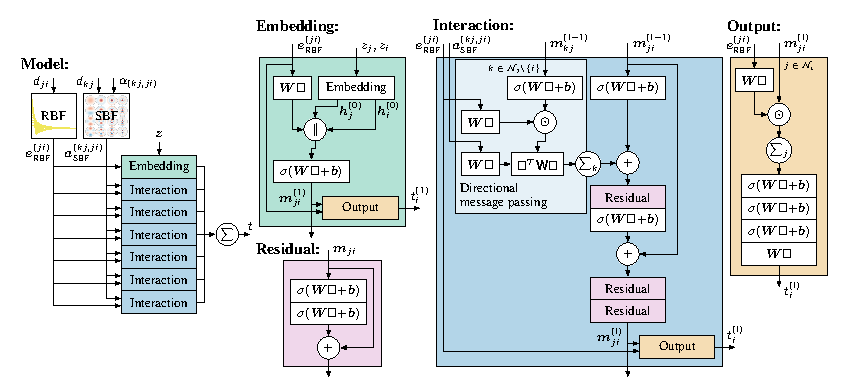
\includegraphics[]{atomic_simulations/dimenet.pdf}
    \caption{The original DimeNet architecture as depicted in \cite*{DBLP:journals/corr/abs-2003-03123}.}
    \label{fig:dimenet}
\end{figure}

DimeNet++ \cite{https://doi.org/10.48550/arxiv.2011.14115} is an upgraded version of 
DimeNet that increases the efficiency of training without impacting the quality of results. 
These improvements include replacing the bilinear layer in the directional message passing 
step by a simpler Hadamard product, downprojecting the embeddings into lower dimensions in
computation-intensive parts of the model and upproject them back to the original dimensions 
after these layers, and using less interaction layers.

\subsubsection{GemNet}
\label{subsubsec:gemnet}

Gasteiger et al. proposed GemNet \cite{https://doi.org/10.48550/arxiv.2106.08903} 
as an improvement over DimeNet and DimeNet++ (see 
\cite{DBLP:journals/corr/abs-2003-03123, https://doi.org/10.48550/arxiv.2011.14115} 
and \ref{subsubsec:dimenet}) in which essentially also quadruplets of nodes are
taken into account. 

Just like DimeNet and DimeNet++, GemNet (\enquote{Geometric Message Passing Neural Network}) takes the positions $\XX$ and atomic numbers 
$\zz$ of a molecule (defined in \eqref{eq:molecule_setup}) as inputs. For
$a, b \in \set{1, \dots, n}$ write
\[
    x_{ab} \: \coloneqq \: \norm{\xx_a - \xx_b}_2 
    \qquad \text{and} \qquad 
    \vec{\xx}_{ab} \: \coloneqq \xx_b - \xx_a
\]
for the distance and relative direction from $\xx_a$ to $\xx_b$ respectively.
\begin{wrapfigure}{r}{0.3\textwidth}
    \centering
    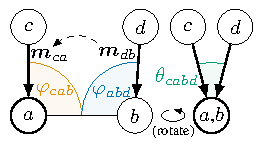
\includegraphics[]{atomic_simulations/gemnet_message_passing.pdf}
\end{wrapfigure}
In GemNet, there are two graphs considered: an interaction graph and an embedding graph.
The molecule's interaction graph does not change during the forward pass of the network and 
two atoms \textit{interact} if their distance is below some 
cutoff $c_{\text{int}}$. In addition to this interaction graph, all atom pairs 
whose distance is below some threshold $c_{\text{emb}}$ are \textit{embedded}---and, thus, edges 
of the embedding graph.

In contrast to DimeNet, quadruplets of 
nodes are now taken into account for message passing: Consider pairwise different $a, b, c, d \in \set{1, \dots, n}$,
where $(x_{ab}, a, b)$ are interacting and $(\_, c, a)$, $(\_, d, b)$ are
embedded. Set
\[
    \varphi_{cab} \: \coloneqq \: 
    \measuredangle \left( \vec{\xx}_{ca}, \vec{\xx}_{ab} \right)
    \qquad \text{and} \qquad
    \varphi_{abd} \: \coloneqq \: 
    \measuredangle \left( \vec{\xx}_{ab}, \vec{\xx}_{db} \right) \text{,}
\]
as well as 
\[
    \phi_{cabd} \: \coloneqq \: \measuredangle \left( \boldsymbol{\Pi} \vec{\xx}_{ca}, \boldsymbol{\Pi} \vec{\xx}_{db} \right),
    \qquad \boldsymbol{\Pi} \: \coloneqq \: \boldsymbol{I}_3 - \vec{\xx}_{ab} \vec{\xx}_{ab}^\top \text{,}
\]
where $\boldsymbol{\Pi}$ is the orthogonal projection onto the orthogonal
complement of $\vec{\xx}_{ab}$.

Similarly to DimeNet, this relative directional information is then represented 
by spherical Fourier-Bessel bases
\[
    \eee_{\text{RBF}}^{(ca)} \: = \: \eee_{\text{RBF}}(x_{ca}), 
    \quad \eee_{\text{CBF}}^{(cab)} \: = \: \eee_{\text{CBF}}(x_{ca}, \varphi_{cab}),
    \quad \eee_{\text{SBF}}^{(cabd)} \: = \: \eee_{\text{SBF}}(x_{ca}, \varphi_{cab}, \phi_{cabd}) 
    \text{.}
\]
After this setup phase, initial node embeddings $\hh_{a}^{(1)}$, edge embeddings 
$\mm_{ca}^{(1)}$ (for each pair $(c, a)$ of nodes that is embedded) and outputs
$t_{a}^{(1)}$ or a global attribute $t^{(1)} = \sum_{a=1}^n t_a^{(1)}$
are computed based on $\zz$ and $\eee_{\text{RBF}}^{(ca)}$. 

The initial input graph can now also be roughly expressed in the
EGN framework (see \ref{subsubsec:egns} and 
\cite{https://doi.org/10.48550/arxiv.2203.09697}) as follows:
\[
    G \: = \: (t^{(1)}, V^{(1)}, E^{(1)}, T^{(1)})
\]
with nodes and edges
\begin{align*}
    V^{(1)} \: &\coloneqq \: \setcomp{\hh_{a}^{(1)}}{a \in \set{1, \dots, n}}, \\
    E^{(1)} \: &\coloneqq \: \setcomp{(\mm_{ca}^{(1)}, c, a)}{c, a \in \set{1, \dots, n}, \: x_{ca} \leq c_{\text{emb}}}
\end{align*}
as well as 3- and 4-way interactions
\begin{align*}
    T^{(1)} \: &\coloneqq \quad \setcomp{(\_, c, a, b)}{c, a, b \in \set{1, \dots, n}, \: x_{ca} \leq c_{\text{emb}}, \: x_{ab} \leq c_{\text{int}}} \\
    &\qquad \cup  \setcomp{(\_, c, a, b, d)}{c, a, b, d \in \set{1, \dots, n}, \: x_{ca} \leq c_{\text{emb}}, \: x_{ab} \leq c_{\text{int}}, \: x_{db} \leq c_{\text{emb}}};
\end{align*}
where the higher-order attributes are handled implicitly (denoted by \enquote{$\_$}) 
based on the node and edge embeddings, are indexed by the involved nodes (contrary to \eqref{eq:higher_order_interact}),
 and all appearing $a, b, c, d$ are assumed to be 
pairwise different.

This input graph is now successively updated in the GN/EGN scheme using a sequence of complex interaction
blocks in which the relative directional information 
$\eee_{\text{RBF}}^{(ca)}$, $\eee_{\text{CBF}}^{(cab)}$, $\eee_{\text{SBF}}^{(cabd)}$ is put to use. 
The complete GemNet architecture as depicted in 
\cite{https://doi.org/10.48550/arxiv.2106.08903} can be seen in Figure~\ref{fig:gemnet}.

\begin{figure}[H]
    \centering
    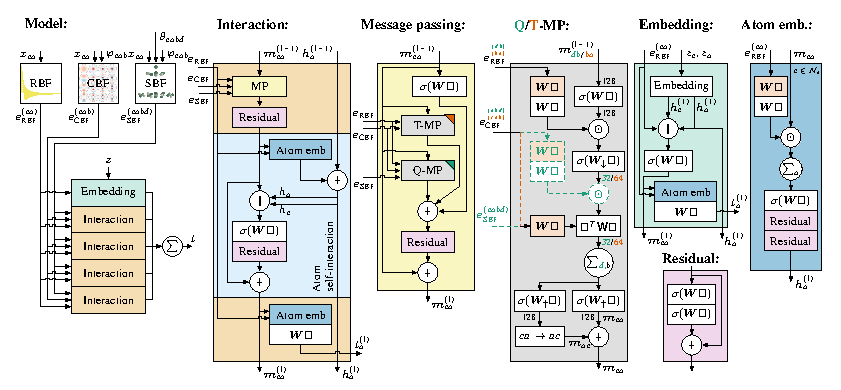
\includegraphics[]{atomic_simulations/gemnet.pdf}
    \caption{Complete architecture of GemNet as depicted in \cite[Appendix F]{https://doi.org/10.48550/arxiv.2106.08903}.}
    \label{fig:gemnet}
\end{figure}


